\documentclass[letterpaper,11pt]{article}
\oddsidemargin -1.0cm \textwidth 17.5cm

\usepackage[utf8]{inputenc}
\usepackage[activeacute,spanish, es-lcroman]{babel}
\decimalpoint
\usepackage{amsfonts,setspace}
\usepackage{amsmath}
\usepackage{amssymb, amsmath, amsthm}
\usepackage{comment}
\usepackage{float}
\usepackage{amssymb}
\usepackage{dsfont}
\usepackage{anysize}
\usepackage{multicol}
\usepackage{enumerate}
\usepackage{graphicx}
\usepackage[left=1.5cm,top=2cm,right=1.5cm, bottom=1.7cm]{geometry}
\setlength\headheight{63pt} 
\usepackage{fancyhdr}
\usepackage{multicol}
\usepackage{hyperref}
\usepackage{wrapfig}
\usepackage{subcaption}
\usepackage{siunitx}
\usepackage{cancel}
\usepackage{mdwlist}
\usepackage{svg}
\pagestyle{fancy}
\fancyhf{}
\renewcommand{\labelenumi}{\normalsize\bfseries P\arabic{enumi}.}
\renewcommand{\labelenumii}{\normalsize\bfseries (\alph{enumii})}
\renewcommand{\labelenumiii}{\normalsize\bfseries \roman{enumiii})}


\fancyhead[L]{Centro de estudiantes de Plan Com\'un \\ Facultad de Ciencias F\'isicas y Matem\'aticas \\ Universidad de Chile \\ Introducci\'on a la F\'isica Cl\'asica FI1000 2022-1}
\fancyhead[R]{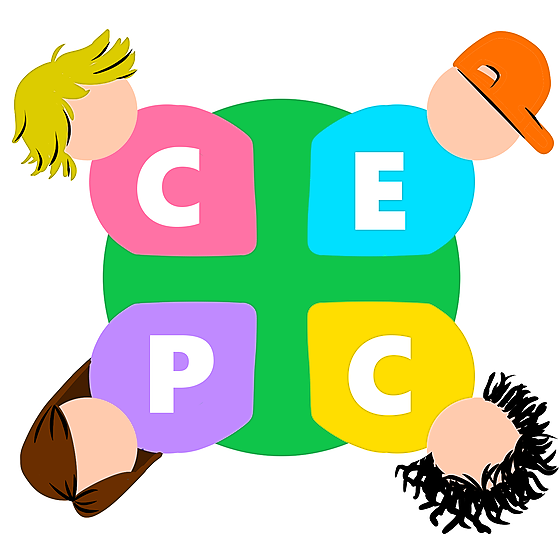
\includegraphics[width=0.11\linewidth]{2022-1/img/cepc/cepc.png}}

\begin{document}

\begin{center}
	\LARGE\textbf{Tutoría movilizada 2 Introducción a la Física Clásica}\\
	\large{Tutor: Alejandro S. Cartes}
\end{center}

\vspace{-1cm}
\begin{enumerate}\setlength{\itemsep}{0.4cm}

\rfoot[]{pág. \thepage}

\item[]

\item
\begin{multicols}{2}
    Un bloque de masa $m$ está apoyado sobre la superficie de una cuña, que forma un ángulo $\alpha$ con la horizontal. La superficie de contacto entre ambas superficies está caracterizada por coeficientes de roce estático $\mu_e$ y cinético $\mu_c$, que son suficientemente grandes de manera que el bloque no desliza si la cuña está inmóvil. Mediante una cuerda, la cuña es forzada a moverse hacia la derecha con una aceleración constante $a_0$, tal como se muestra en la figura. 

    \columnbreak

    \begin{figure}[H]
        \centering
        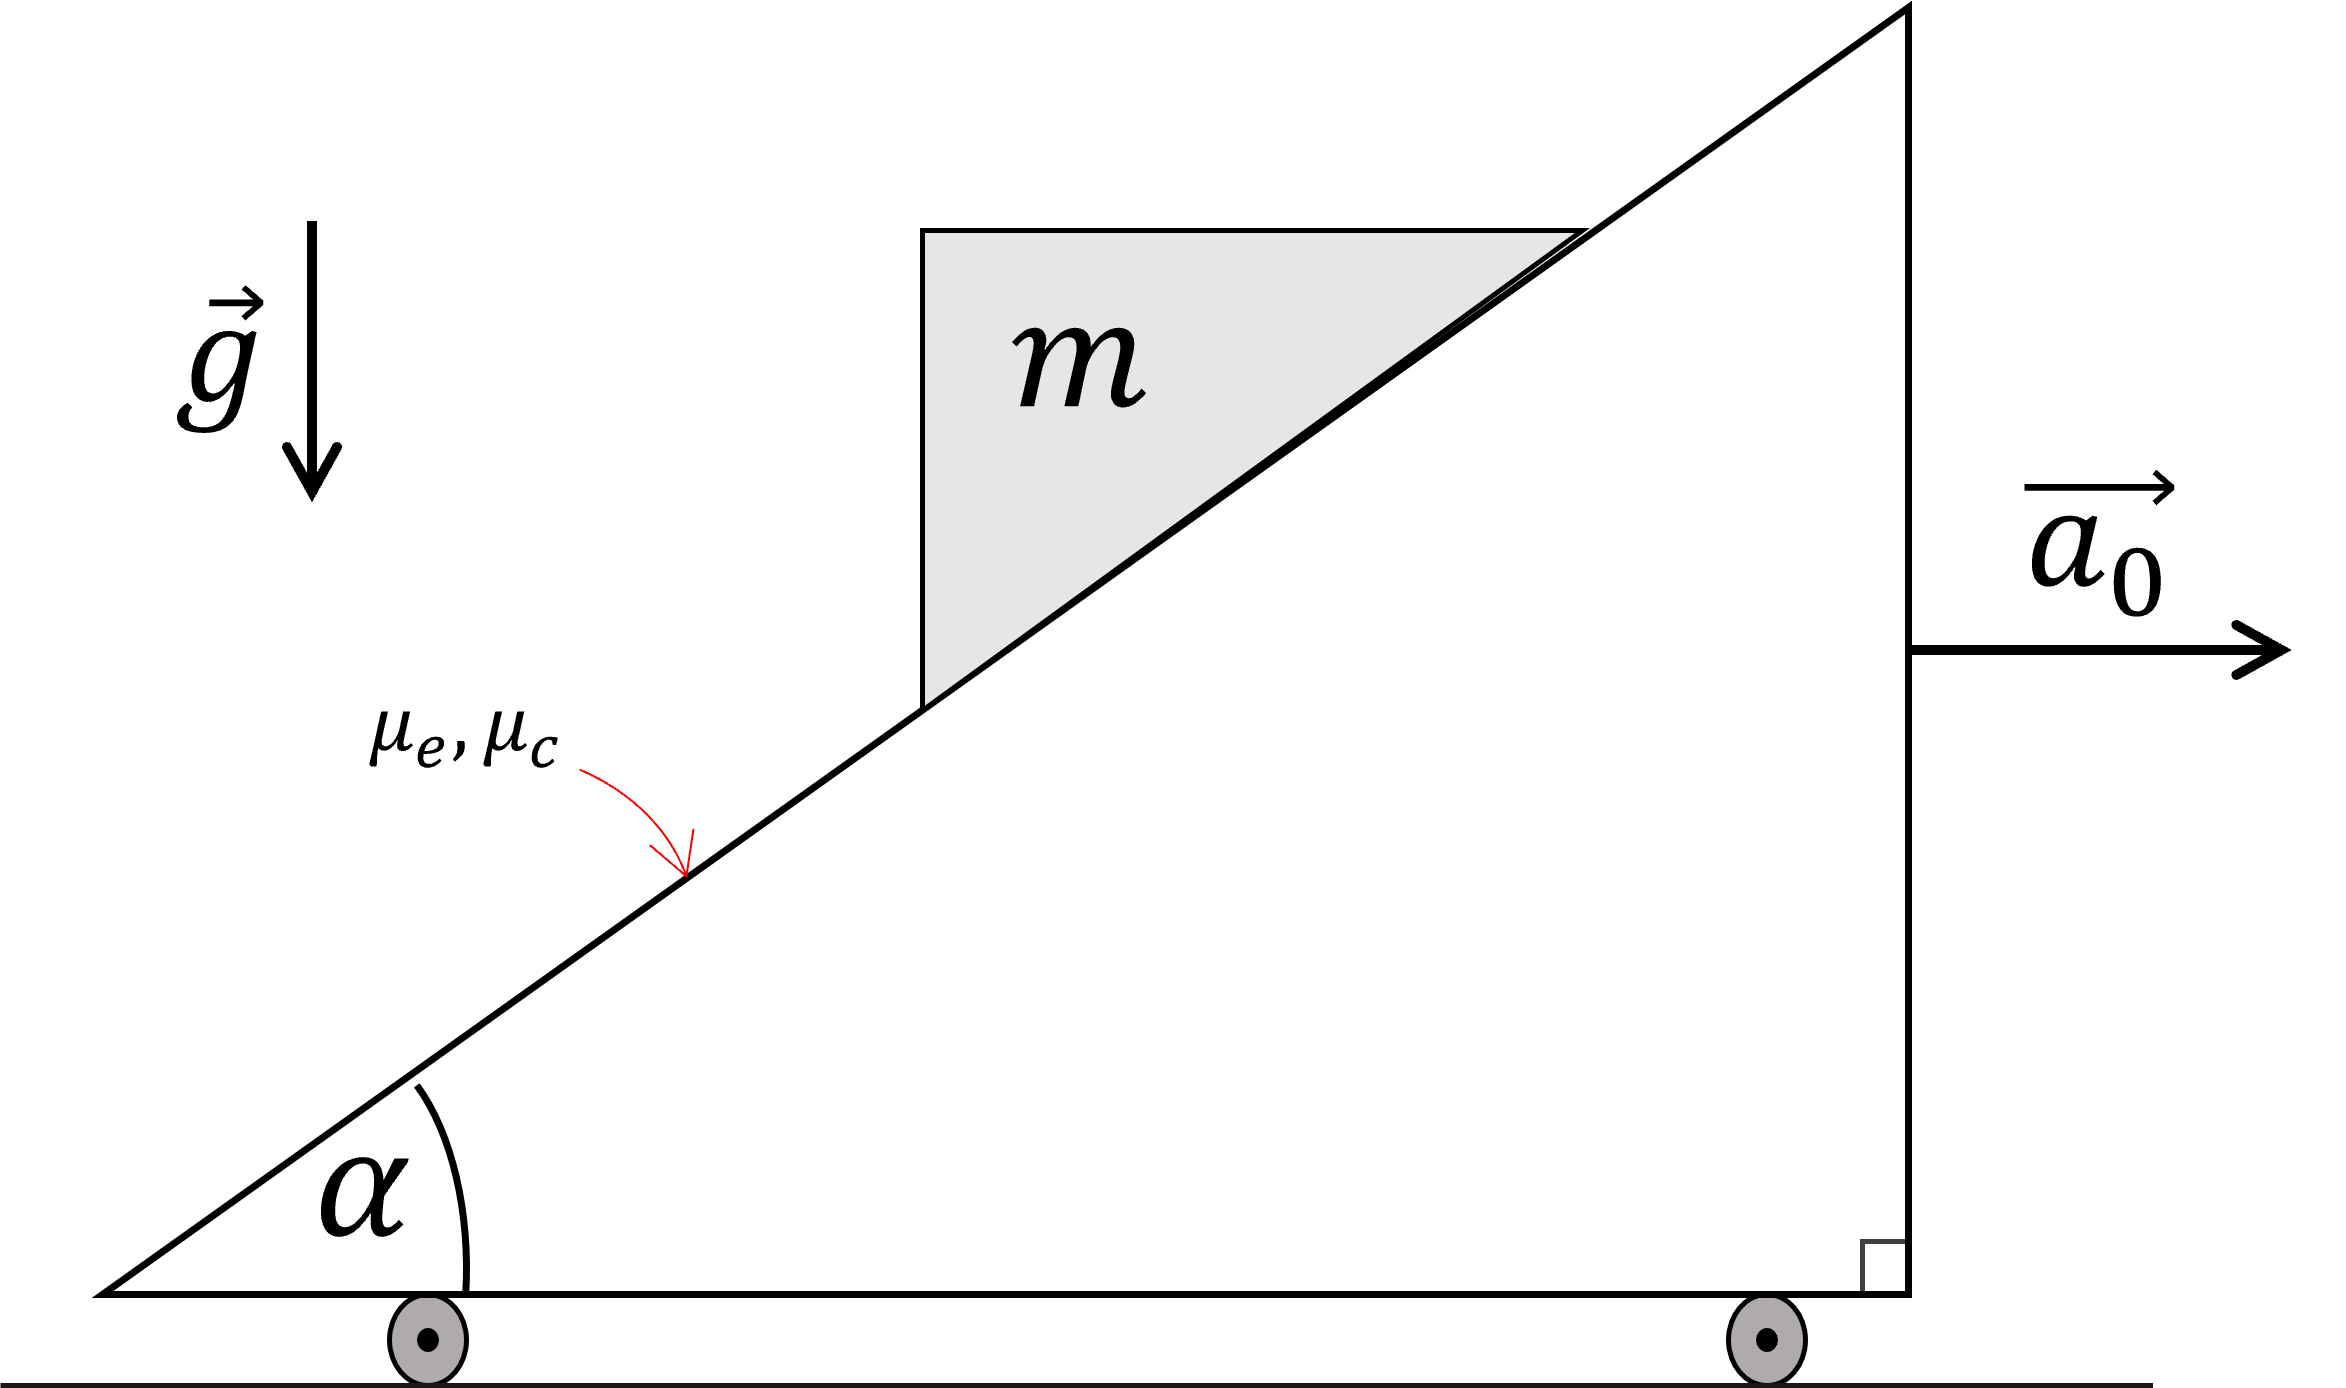
\includegraphics[width=0.8\linewidth]{2022-1/img/cepc/masa cunia.png}
    \end{figure}
\end{multicols}
    \begin{enumerate}
        \item Determine el valor mínimo de $a_0$ de manera que el bloque empieza a deslizar sobre la cuña.
        
        \item Si se cumple la condición encontrada en la parte anterior, calcule la componente vertical de la aceleración del bloque
    \end{enumerate}
    

\item Dos esferas están unidas por una cuerda ideal que pasa por dos orificios de una mesa horizontal, con la geometría que se muestra en la figura. Una de las esferas, de masa $\lambda m$, cuelga verticalmente. Mientras que la otra esfera, de masa $m$, gira con velocidad angular constante $\omega$ a una distancia $L$ de la mesa. Determine el valor de $\omega$ y el ángulo $\beta$ si la esfera de masa $\lambda m$ está quieta, ¿qué condición debe cumplir $\lambda$ para que sea posible el sistema descrito?.

\begin{figure}[H]
    \centering
    \svgpath{../../2021-2/img/aux4}
    \includesvg[width=0.45\linewidth]{mesa.svg}
\end{figure}

% https://drive.google.com/file/d/1l1oERtv7ulScv3sL-zs049YW2KtWyjLd/view?usp=sharing

\item Un cubo de masa $M$, que posee un hueco esférico de radio $R$, descansa en un orificio de superficies rectas y sin roce. Al interior del cubo hay una bolita de masa $m$ que gira sin ayuda externa en un trayecto circunferencial que pasa por el punto más bajo del hueco. En tal punto la bolita tiene rapidez $v_0$.

    \begin{enumerate}
        \item Determine la fuerza de contacto bolita-superficie en función del ángulo $\theta$ medido con respecto la vertical
        
        \item Determine el rango $v_0$ que garantice que la bolita nunca pierda contacto con la superficie, ni el cubo pierda contacto con el fondo del orificio.
    \end{enumerate}
    
\begin{figure}[H]
    \centering
    \svgpath{../../2021-2/img/aux4}
    \includesvg[width=0.35\linewidth]{cubo.svg}
\end{figure}

% https://drive.google.com/file/d/1bEBSW7gOW0OLIviY-kFC8-d5An_9djw6/view?usp=sharing

% Para imágenes vectoriales -> el texto tiene que estar en LaTeX
% \begin{figure}[htbp]
%   \centering
%   \svgpath{../Imagenes/ejercicios}  -> .. irse pa'trás 
%   \includesvg{ej5.svg}
% \end{figure}

\end{enumerate}
\end{document}
